\section{Introduzione} 
\subsection{L'azienda}
\begin{figure}[H]
\begin{center}

\includegraphics[height=1.6cm]{Pics/logo_moku.jpg}
\caption{Logo dell'azienda ospitante - Moku S.r.l.}
\end{center}
\end{figure}
Moku S.r.l è una startup nata nel 2013 e situata in H-Farm. 
L'organizzazione del lavoro è supportata dalla suite Atlassian che offre un servizio cloud per la gestione dei compiti e dei progetti.
L'azienda lavora a stretto contatto con il cliente definendo requisiti, user experience dei prodotti realizzati ed opportunità di business.
Obiettivo primario dell'azienda è la qualità del software e l'utilizzo di tecnologie recenti poiché l'alto coefficiente innovativo dei prodotti realizzati rende necessaria una costante manutenzione che si vuole sia il più agevole possibile.

\subsubsection{Origine}
Il nome della startup, in hawaiiano, significa \textit{isola}. Questo perché l'idea iniziale era una applicazione web per studenti dove un \textit{"moku"} era visto come uno spazio personale (un’isola), ma allo stesso tempo uno spazio di collaborazione, rappresentando un \textit{arcipelago} di isole collegate tra loro.
In origine si basava sulla realizzazione di una applicazione il cui uso era riservato principalmente agli studenti. Ad ogni utente era data la possibilità di caricare i propri documenti in diverse tipologie di formato. Una volta aperti, era possibile prendere degli appunti su un layer posto sopra al documento caricato. Questo può essere condiviso con i propri collaboratori. Era anche possibile registrare la lezione e mettere delle note anche alla traccia audio, la quale si poteva sincronizzare con un particolare documento.
\subsubsection{Evoluzione}
Ora le attività dell'azienda si concentrano nella consulenza IT, in particolare nella realizzazione di software innovativo a supporto delle esigenze concrete dei clienti. Il progetto da me svolto è un chiaro esempio di questo mutamento, infatti il prodotto finito risulterà di completa proprietà di un'azienda esterna.  \\ Ora l'azienda, quindi, sviluppa solo marginalmente software proprietario, ma sviluppa principalmente su commissione di aziende esterne.

\subsection{Organizzazione del lavoro}
\begin{figure}[H]
\begin{center}
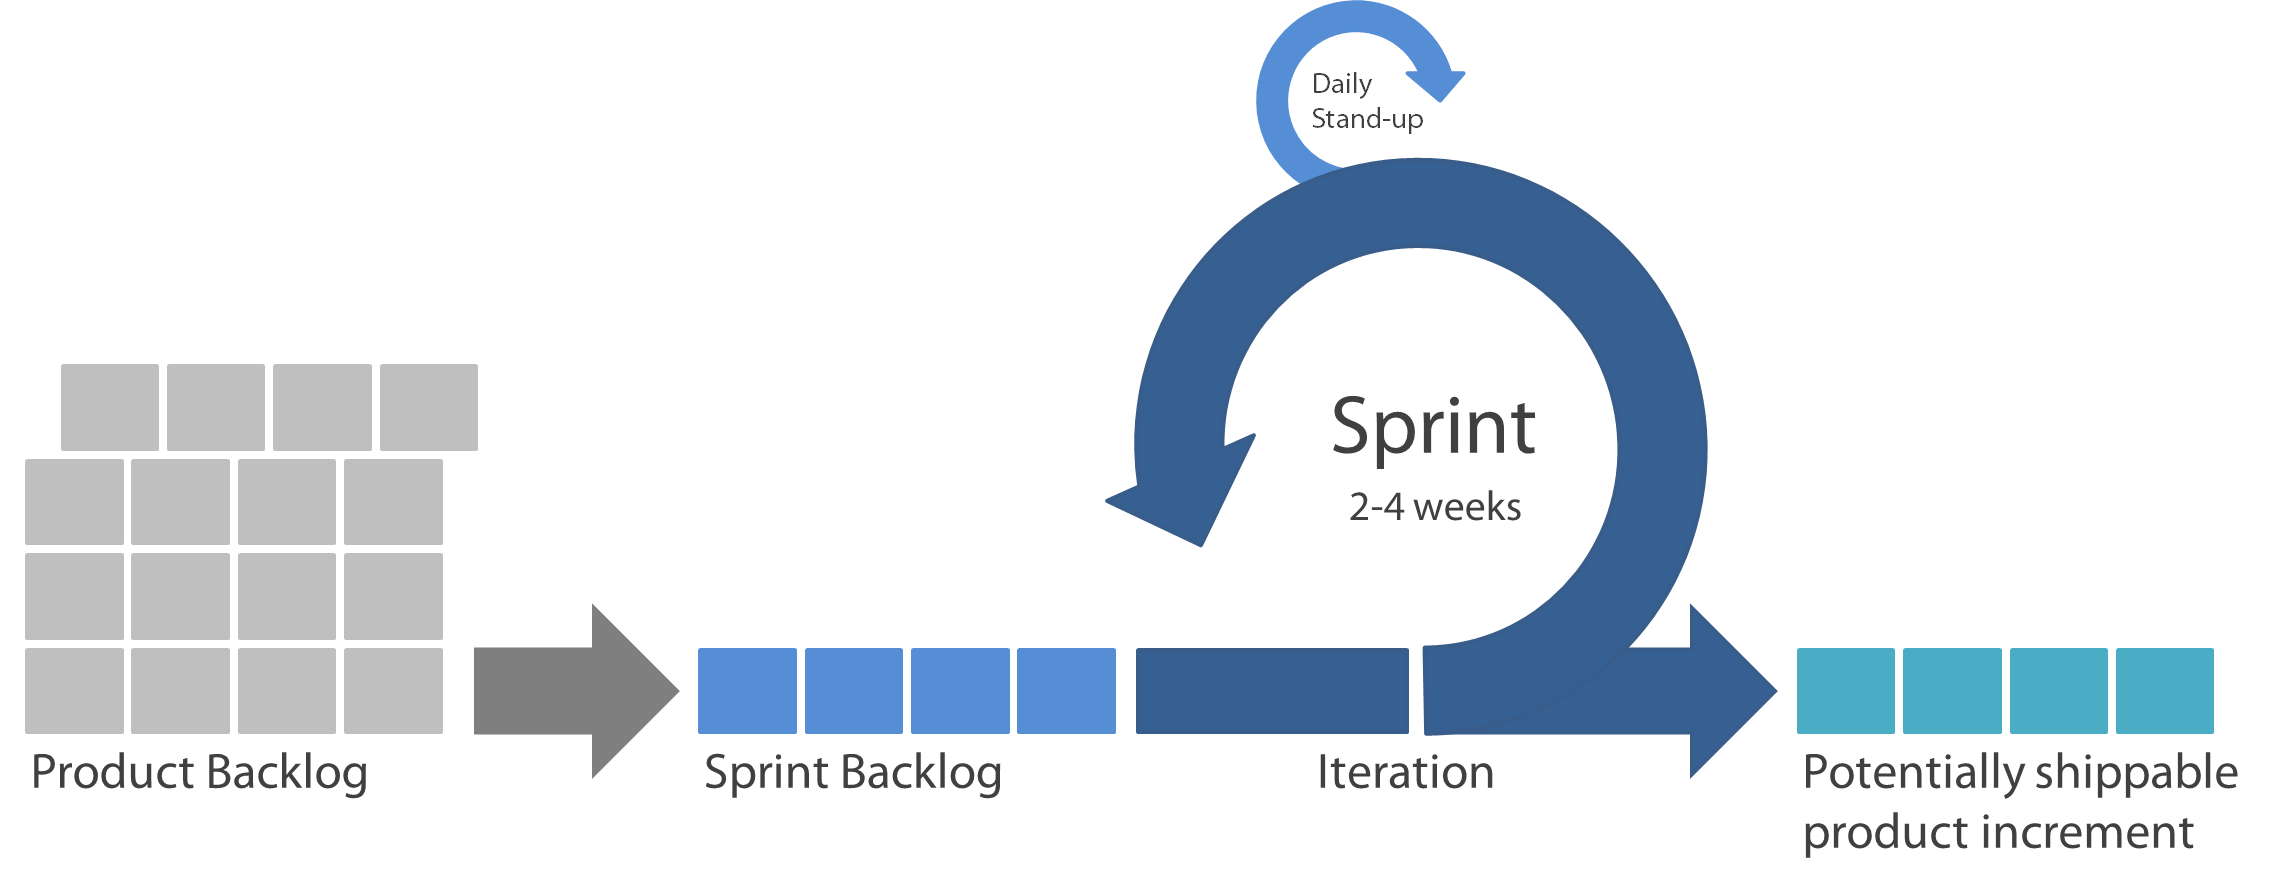
\includegraphics[width=12cm]{Pics/scrum.png}
\caption{Metodo agile scrum.}
\end{center}
\end{figure}
All'interno dell'azienda il lavoro viene organizzato secondo il metodo agile scrum.  \\
Il modello agile scrum prevede la suddivisione di un progetto in blocchi detti \textit{Sprint} ognuno dei quali deve produrre un avanzamento del software. Prevede, inoltre la suddivisione dei compiti in \textit{task}, che possono essere visti come una attività abbastanza piccola da essere svolta da una sola persona nell'arco di 4/8 ore. È previsto un rapporto a stretto contatto con il cliente e la pianificazione di frequenti meeting con la funzione di punti di controllo, dove verificare lo stato di avanzamento del progetto rispetto a quanto atteso.
È stato scelto questo modello poiché l'azienda sviluppa in maggioranza prodotti innovativi, quindi con tecnologie in evoluzione, e soggetti a continue variazioni dei requisiti rendendo necessaria un meccanismo di controllo flessibile. Nello specifico del progetto in analisi, la continua variazione delle norme di legge in vigore provoca continui mutamenti nell'implementazione del software ed un rapporto a stretto contatto con il cliente diventa indispensabile al fine di garantire la conformità del servizio.

\subsection{Strumenti a supporto dell'organizzazione del lavoro}
\subsubsection{Atlassian Suite}
\begin{figure}[H]
\begin{center}

\includegraphics[height=1.1cm]{Pics/atlassian_logo.png}
\caption{Logo della suite Atlassian}
\end{center}
\end{figure}
Per l'organizzazione del lavoro, ci si è appoggiati alla suite offerta da Atlassian, che fornisce tutti gli strumenti necessari alla gestione di codice e compiti. \\
Fa seguito l'elenco degli strumenti utilizzati a supporto delle principali necessità.

\subsubsection{Jira - Gestione dei Task e Sprint }
\begin{figure}[H]
\begin{center}

\includegraphics[height=1.4cm]{Pics/jira_logo.png}
\caption{Logo di Jira}
\end{center}
\end{figure}

Per la gestione dei \textit{Task} e degli \textit{Sprint} è stato utilizzato il software Jira della suite Atlassian.\\
Esso permette di creare ed assegnare i task alle persone le quali possono annotare il numero di ore dedicate ad ogni specifico task. È possibile inoltre avere una visione d'insieme dello sprint corrente e dei precedenti, pianificando anche i successivi.
È anche possibile collegare i task presenti su Jira con i \textit{commit} presenti su Bitbucket facendo riferimento nel testo del \textit{commit} al codice identificativo del \textit{task} tenendo sotto controllo l'evoluzione del codice per ogni \textit{task}.


\subsubsection{Confluence - Gestione  della documentazione}

\begin{figure}[H]
\begin{center}

\includegraphics[height=0.7cm]{Pics/confluence_logo.jpeg}
\caption{Logo di Confluence}
\end{center}
\end{figure}

Per la gestione della documentazione su norme aziendali e prodotti realizzati, viene utilizzato il software Confluence. Esso fornisce usa sorta di wiki integrato con tutte le applicazioni della suite collegata al progetto. Qui viene stesa la documentazione inerente a tutte le fasi del ciclo di vita del prodotto.

\subsubsection{Bitbucket - Versionamento}
\begin{figure}[H]
\begin{center}

\includegraphics[height=1cm]{Pics/bitbucket_logo.png}
\caption{Logo di Bitbucket}
\end{center}
\end{figure}

Per quanto riguarda il versionamento, viene utilizzato il servizio Bitbucket della suite. Esso utilizza \texttt{git} per la gestione del repository. 
 Per agevolare la cooperazione è stato adottato l'approccio \textbf{git-flow}. 

\subsubsection{Slack - Comunicazione}

\begin{figure}[htbp]
\begin{center}

\includegraphics[height=1cm]{Pics/slack_logo.png}
\caption{Logo di Slack}
\end{center}
\end{figure}

Per quanto riguarda la comunicazione interna ai membri dell'azienda è stato scelto di utilizzare il software gratuito Slack. 
Si tratta di un sistema di messaggistica che distingue le comunicazioni dirette a persone da quelle dirette a canali inerenti ad un particolare argomento. Le norme aziendali prevedono la creazione di un canale per ogni progetto.
Slack mette a disposizione anche un meccanismo di condivisione di file e, caratteristica essenziale, mantiene uno storico di tutti i messaggi di tutte le conversazioni al fine di mantenere un tracciamento delle comunicazioni interne. 
È fornita dal software anche una efficiente funzionalità di ricerca per recuperare le comunicazioni o i contenuti condivisi.
\subsubsection{Errbit - Rilevazione degli errori }

\subsubsection{Airbrake - Rilevazione e notifica degli errori}

\begin{figure}[htbp]
	\begin{center}
		
\includegraphics[height=1.6cm]{Pics/airbrake_logo.png}
		\caption{Logo di Airbrake}
	\end{center}
\end{figure}
\hl{todo rivedere}
Airbrake è uno strumento per la rilevazione e gestione degli errori dotato di un sistema di notifiche push centralizzato. \\
La sua caratteristica principale è quella di centralizzare la gestione delle notifiche permettendo un'accurata gestione dei flussi di spedizione dei messaggi e degli ambienti monitorati (sviluppo, staging, produzione). \\ 
Esso ha bisogno di essere installato su un server dove mantiene dei listener pronti a catturare i messaggi di errore provenienti dall'applicazione alla quale è collegato.\\
Per ogni errore rilevato, vengono resi disponibili su una pagina web le informazioni relative alla tipologia dell'errore, il backTrace, l'utente per il quale è avvenuto, ed i parametri sottomessi alla pagina in analisi.\\
Nello stage è stato fatto uso di questo framework nel server in produzione per essere a conoscenza con esattezza delle criticità del prodotto realizzato in modo da essere reattivi nella risoluzione dei bug rilevati.\\
Airbrake è stato configurato in modo tale che le notifiche provenienti dal monitoraggio dell'ambiente di produzione siano spedite ad un canale di Slack appositamente creato.


\cleardoublepage
\section{Il progetto di Stage}
Il progetto di stage consiste nell'estensione di un software web based, già sviluppato in azienda, a supporto delle aziende che intendono avvalersi dell’asseverazione in ambito della sicurezza sul lavoro, in particolare nel settore edilizio. \\
Con asseverazione si intende una scelta volontaria di una impresa edile al fine di dimostrare l'impegno per la prevenzione, salute e sicurezza nei luoghi di lavoro. Opera mediante la certificazione di conformità dei modelli di organizzazione e gestione aziendali e mediante visite a campione nei cantieri. L'asseverazione offre benefici economici alle aziende che la richiedono e garantisce efficacia esimente rispetto alla responsabilità amministrativa delle imprese.\\
Il software si pone come obiettivo la possibilità di fornire in ogni momento una fotografia dello stato della sicurezza in azienda, al fine di agevolarne il mantenimento nel tempo.\\
All'inserimento di nuove informazioni, verranno generate nuove domande, scadenze o vincoli. Se i risultati non sono conformi alle norme vigenti, verranno generati degli allarmi, che scompariranno solo nel momento in cui la violazione del vincolo che rappresentano non sia più verificata. \\
Dal punto di vista tecnico viene utilizzato un sistema esperto per mappare le norme in tema di sicurezza, individuare i punti deboli dell’azienda, ricordare al responsabile le scadenze, conservare ed indicizzare il patrimonio documentale in ambito sicurezza.
Il sistema ha una funzione proattiva e dinamica, variando gli allarmi in base alla variazione delle norme e allo stato dell’azienda (es. al crescere o diminuire del numero dei dipendenti, al variare della superficie delle sedi aziendali, dei cantieri...). La webapp si comporta quindi come un consulente digitale per l’azienda, aiutandola a mantenere aggiornato il suo modello di sicurezza e a rispettarlo.
Questo le permette all’azienda asseverata di accedere a significativi premi INAIL, di ottenere punti in graduatoria in bandi pubblici e di sollevare il datore di lavoro da responsabilità penali in caso di infortuni legati ad una mala gestione della sicurezza.\\
\hl{
La filosofia generale del progetto prevede che sia  sempre possibile inserire i dati senza blocchi dettati dai vincoli di legge, in modo da evidenziare eventuali non conformità con allarmi al fine di risolverle.
}
\subsection{Il prodotto esistente}

Il progetto è in una fase di sviluppo avanzato (versione alpha).
Alla data di inizio dello stage, il software supporta le aziende con i codici \gls{ATECO}\G\ in ambito edilizio, permette l’inserimento di informazioni su sedi, cantieri, dipendenti, organigramma aziendale e la gestione di abitabilità, certificato prevenzione incendi e della documentazione che emerge dal \gls{DVR}\G.
Vengono poste all'utente più di 400 domande per individuare lo stato di sicurezza. \\ 
Il sistema esperto è funzionante, ma va irrobustito e vanno implementate le regole opportune per individuare le criticità nei dati inseriti dall'utente.


\subsection{Obiettivi dello stage}

Il team ha l’obiettivo di rilasciare una versione beta del software entro la fine del 2015 e quindi procedere al primo test con l’utente finale, una importante azienda del settore edilizio, già  individuata.
Durante lo stage sono stati posti i seguenti obiettivi:
\begin{itemize}
\item Analisi di alcune logiche del sistema esperto in coordinamento con il cliente ed il consulente della sicurezza;
\item Progettazione delle funzionalità individuate nella fase di analisi;
\item Implementazione del risultato del punto precedente;
\item Stesura della documentazione relativa al codice prodotto;
\item Rendere il sistema più efficace, semplice ed usabile da parte di un utente competente in materia di sicurezza.
\end{itemize}
